\documentclass[letterpaper, 10 pt, journal, twoside]{IEEEtran}

\usepackage{cite}
\usepackage{amsmath,amssymb,amsfonts}
\usepackage{amsthm}
\renewcommand\qedsymbol{$\blacksquare$}
\usepackage{graphicx}
\usepackage{booktabs}
\usepackage{multirow}
\usepackage{makecell}
\usepackage{xcolor}
\usepackage{url}
\usepackage{algorithm}
\usepackage{algorithmic}
\usepackage{balance}

\hyphenation{op-tical net-works semi-conduc-tor IEEE-Xplore}

% Theorem environments
\newtheorem{proposition}{Proposition}
\newtheorem{remark}{Remark}

% Placeholders for results / numbers that are not available yet (shown in red)
\newcommand{\tbd}[1]{\textcolor{red}{#1}}
% Framed placeholder for figures that still have to be drawn
\newcommand{\figbox}[2]{\fbox{\parbox[c][#2][c]{0.94\linewidth}{\centering\footnotesize\textcolor{red}{#1}}}}

% Shorthand macros
\DeclareMathOperator{\tr}{tr}
\newcommand{\bp}{\mathbf{p}}
\newcommand{\bx}{\mathbf{x}}
\newcommand{\bd}{\mathbf{d}}
\newcommand{\bg}{\mathbf{g}}
\newcommand{\bq}{\mathbf{q}}
\newcommand{\bs}{\mathbf{s}}
\newcommand{\bo}{\mathbf{o}}
\newcommand{\bu}{\mathbf{u}}
\newcommand{\JF}{J_{\mathrm{F}}}
\newcommand{\JA}{J_{\mathrm{AC}}}
\newcommand{\JFbar}{\bar{J}_{\mathrm{F}}}

\begin{document}

\title{Ambiguity-Aware Active Localization for Terrain-Referenced Navigation of AUVs Using Autocorrelation-Informed MPPI}

\author{Kiyong~Park$^{1,\dagger}$, Dongwook~Lee$^{2,\dagger}$, and Jinwhan~Kim$^{1,*}$% <-this % stops a space
\thanks{Manuscript received: Month, Day, Year; Revised Month, Day, Year; Accepted Month, Day, Year.}%
\thanks{This paper was recommended for publication by Editor Editor A. Name upon evaluation of the Associate Editor and Reviewers' comments.}%
\thanks{This work was supported by \tbd{[funding agency and grant number]}.}%
\thanks{$^{\dagger}$Kiyong Park and Dongwook Lee contributed equally to this work. $^{*}$Corresponding author: Jinwhan Kim.}%
\thanks{$^{1}$Kiyong Park and Jinwhan Kim are with the Department of Mechanical Engineering, Korea Advanced Institute of Science and Technology (KAIST), Daejeon 34141, Republic of Korea (e-mail: qkrrldyd777@kaist.ac.kr; jinwhan@kaist.ac.kr).}%
\thanks{$^{2}$Dongwook Lee is with the Robotics Program, Korea Advanced Institute of Science and Technology (KAIST), Daejeon 34141, Republic of Korea (e-mail: dongwooklee1201@kaist.ac.kr).}%
\thanks{Digital Object Identifier (DOI): see top of this page.}
}

\markboth{IEEE Robotics and Automation Letters. Preprint Version. Accepted Month, Year}%
{Park \MakeLowercase{\textit{et al.}}: Ambiguity-Aware Active Localization for Terrain-Referenced Navigation of AUVs}

\maketitle

%% ---------------------------------------------------------------
%%  ABSTRACT
%% ---------------------------------------------------------------
\begin{abstract}
Terrain-referenced navigation (TRN) allows autonomous underwater vehicles (AUVs) to bound dead-reckoning drift by matching altimeter measurements to a bathymetric map, but its reliability depends strongly on the path the vehicle takes. When the initial position uncertainty is large, repetitive or elongated seafloor features such as sand waves and slope bands produce several equally plausible position hypotheses, and the filter may converge to a wrong one. Conventional information-aware planners predict the localization performance from the terrain gradient, i.e., the Fisher information, which is valid only for small uncertainty and is therefore overconfident on such terrain. This paper presents an ambiguity-aware active localization framework that integrates an autocorrelation-based terrain information model into model predictive path integral (MPPI) control. The information model evaluates the local terrain autocorrelation under the current belief size and retains only the information that remains unambiguous, reducing to the Fisher information in the small-uncertainty limit. Precomputed at multiple belief scales, it is embedded in a belief-dependent covariance prediction along rollouts of an AUV maneuvering model, and the planner generates heading-rate commands that trade off the terminal uncertainty and the travel time. Monte Carlo simulations with a six-degree-of-freedom REMUS~100 model on eight real bathymetric maps show that the proposed method achieves a mission success rate of 97.5\%, compared with 68.8--92.1\% for straight-line, A*-based, and Fisher-information-based MPPI baselines and \tbd{XX}\% for a particle-entropy-based MPPI baseline.
\end{abstract}

\begin{IEEEkeywords}
Marine robotics, localization, motion and path planning, planning under uncertainty.
\end{IEEEkeywords}

%% ---------------------------------------------------------------
%%  SECTION I -- INTRODUCTION
%% ---------------------------------------------------------------
\section{Introduction}
\label{sec:intro}
\IEEEPARstart{A}{utonomous} underwater vehicles (AUVs) are increasingly deployed for seabed survey, environmental monitoring, and subsea infrastructure inspection, often over long distances without access to the global navigation satellite system (GNSS). Without external position fixes, the dead-reckoning (DR) solution obtained from an inertial navigation system and a Doppler velocity log (DVL) drifts without bound~\cite{paull2014auv}. Terrain-referenced navigation (TRN) bounds this drift by comparing onboard seafloor measurements with a prior bathymetric map~\cite{bergman1999terrain, carreno2010survey, melo2017survey}, and it can be realized even with a single-beam altimeter that most AUVs already carry~\cite{kim2014nonlinear, claus2015terrain, salavasidis2019terrain}. TRN therefore removes the need to surface for GNSS fixes or to deploy acoustic beacons, which greatly improves the operational efficiency of AUVs.

However, the performance of TRN is determined not only by the estimator but also by the terrain the vehicle traverses, and reliable TRN remains challenging due to several coupled factors. First, the initial position uncertainty after a long DR transit or a dive can reach tens of meters, which is comparable to or larger than the characteristic length of many seafloor features. Second, a single-beam altimeter provides only one scalar measurement per ping, so the position components that become observable depend on the direction in which the vehicle crosses the terrain. Third, natural seafloors frequently contain repetitive or elongated features such as sand waves, linear stripes, and slope bands. On such terrain, several position hypotheses explain the measurements equally well, and the particle filter (PF) can converge to a wrong hypothesis while reporting a small covariance, resulting in a large undetected error at the destination. Therefore, the vehicle must actively select a path that provides information that is not only abundant but also unambiguous at its current level of uncertainty.

Information-aware path planning has been studied to improve localization by steering the vehicle toward informative regions~\cite{fox1998active, prentice2009belief, hausler2013cooperative, zhang2019beyond}. Most of these approaches quantify the information by the gradient of the measurement model, i.e., the Fisher information, and predict the localization error through the Cram\'{e}r--Rao bound~\cite{tichavsky1998posterior}. This prediction is accurate once the belief is narrower than the terrain features, but it is overconfident when the uncertainty is large, because steep but repetitive terrain yields large Fisher information even though its features cannot be told apart. Particle-based information measures avoid this approximation~\cite{hoffmann2010mobile, ryan2010particle}, but their cost grows with the number of particles and hypothetical measurements, which is prohibitive when hundreds of candidate trajectories must be evaluated at every replanning step. Moreover, unambiguous terrain often lies away from the direct route, so the planner must also account for the vehicle dynamics and the travel time when deciding whether a detour pays off.

Motivated by these observations, this paper proposes an ambiguity-aware active localization framework for TRN that integrates an autocorrelation-based terrain information model into model predictive path integral (MPPI) control~\cite{williams2017model, williams2018information}. The information model evaluates how similar the local terrain appears under a position offset, combines this autocorrelation with the current belief size, and retains only the information that remains unambiguous. Because the model depends only on the map and the belief size, it is precomputed at several belief scales and looked up at the cost of a Fisher information map. The MPPI planner embeds the model in a belief-dependent covariance prediction along rollouts of an AUV maneuvering model and directly generates heading-rate commands that trade off the terminal uncertainty and the travel time. As a result, the vehicle first visits terrain that is unambiguous at the current uncertainty and exploits repetitive features only after its belief has become narrower than their period, as illustrated in Fig.~\ref{fig:concept}.

\begin{figure}
  \centering
  % TODO: concept figure. (a) sand-wave terrain (S4 or S5) with the direct route, (b) gradient Fisher information map,
  %       (c) J_AC at sigma = 50 m and (d) at sigma = 5 m, with Fisher-MPPI vs AC-MPPI tracks overlaid.
  \figbox{Fig.~1 placeholder: sand-wave terrain, Fisher information map vs.\ autocorrelation information at $\sigma=50$~m and $\sigma=5$~m, with Fisher-MPPI and AC-MPPI tracks.}{4.2cm}
  \caption{Concept of the proposed ambiguity-aware active localization on a sand-wave field. (a) Bathymetry and the direct route. (b) The gradient-based Fisher information is large over the entire sand-wave field. (c) The proposed autocorrelation information at a belief size of $\sigma = 50$~m retains only the unambiguous terrain, and (d) recovers the Fisher information of the sand waves at $\sigma = 5$~m. The Fisher-based planner loiters over the sand waves, whereas the proposed planner first visits unambiguous terrain and then proceeds to the goal.}
  \label{fig:concept}
  \vspace{-10pt}
\end{figure}

The main contributions of this paper are summarized as follows:
\begin{itemize}
    \item An autocorrelation-based terrain information model is proposed, which quantifies the information that remains unambiguous at the current belief size and reduces to the Fisher information in the small-uncertainty limit.

    \item An MPPI-based active localization framework is developed that embeds the information model into a belief-dependent covariance prediction along rollouts of an AUV maneuvering model, with multi-scale precomputed information maps for real-time planning.

    \item The proposed framework is validated through Monte Carlo simulations with a six-degree-of-freedom (6-DOF) REMUS~100 model on eight real bathymetric maps against straight-line, A*-based, Fisher-based, and particle-entropy-based baselines.
\end{itemize}

The remainder of this paper is organized as follows. Section~II reviews related work. Section~III formulates the active localization problem. Section~IV presents the autocorrelation-based terrain information model, and Section~V describes the proposed MPPI planner. Section~VI presents the simulation results, and Section~VII concludes the paper.

%% ---------------------------------------------------------------
%%  SECTION II -- RELATED WORK
%% ---------------------------------------------------------------
\section{Related Work}
\label{sec:related}
TRN estimates the vehicle position by comparing measured depths or altitudes with a prior bathymetric map~\cite{bergman1999terrain, nygren2004terrain, carreno2010survey, melo2017survey}. Because the measurement function is strongly nonlinear and the posterior is frequently multimodal, PFs have become the standard estimator for TRN~\cite{arulampalam2002tutorial, donovan2012position, teixeira2017robust, kim2018comparison}, and TRN has been demonstrated with multibeam sonars as well as with low-cost altimeters and DVL ranges on long-range AUVs and gliders~\cite{meduna2008low, kim2014nonlinear, claus2015terrain, salavasidis2019terrain}. These studies treat the vehicle path as given, and they consistently report that the accuracy depends on the terrain traversed~\cite{nygren2004terrain, melo2017survey}. In particular, flat, repetitive, or elongated terrain causes slow convergence or convergence to a wrong mode, which a passive estimator cannot resolve on its own.

To predict TRN performance, the posterior Cram\'{e}r--Rao lower bound (PCRLB), i.e., the inverse of the accumulated Fisher information of the terrain gradient, has been widely used~\cite{tichavsky1998posterior, bergman1999terrain}. The PCRLB characterizes the asymptotic accuracy around the true position, but it does not capture large errors caused by competing position hypotheses. In estimation theory, this regime is known as the threshold region, where global bounds such as the Ziv--Zakai bound are governed by the ambiguity of the measurement under a parameter offset rather than by its local curvature~\cite{ziv1969some, bell1997extended}. In TRN, the corresponding ambiguity is determined by how similar the terrain appears under a position offset, i.e., by its autocorrelation, which also underlies correlation-based terrain matching~\cite{nygren2004terrain}. These results indicate that a terrain information measure for planning should account for both the local gradient and the ambiguity at the current level of uncertainty.

Active localization selects actions that reduce the localization uncertainty~\cite{fox1998active}. Belief-space planners propagate a Gaussian belief with an extended Kalman filter or Fisher information and optimize the expected covariance~\cite{prentice2009belief, vandenberg2011lqg, bry2011rapidly, indelman2015planning}, and perception-aware planners and controllers embed Fisher-information-based localization costs into path planning or receding-horizon optimization~\cite{zhang2019beyond, falanga2018pampc}. For TRN, path planners steer the vehicle over terrain with high information content~\cite{hausler2013cooperative}, optimize waypoints for the Monte Carlo probability of reaching the goal~\cite{krukowski2016waypoint}, or select actions that discriminate between position hypotheses of a PF~\cite{fairfield2008active}. Gaussian and Fisher-based predictions are computationally efficient but inherit the local nature of the Fisher information, whereas particle-based information measures~\cite{hoffmann2010mobile, ryan2010particle} and Monte Carlo evaluation~\cite{krukowski2016waypoint} capture multimodality at a cost that grows with the number of particles, simulated measurements, and candidate paths~\cite{hollinger2014sampling}. MPPI control~\cite{williams2016aggressive, williams2017model, williams2018information} optimizes arbitrary nonsmooth costs over sampled rollouts of nonlinear dynamics and is therefore attractive for active localization, provided that the information cost of each rollout can be evaluated in real time. The proposed framework brings these aspects together: an ambiguity-aware information model that is as inexpensive to evaluate as a Fisher information map, embedded in an MPPI planner with AUV dynamics.

%% ---------------------------------------------------------------
%%  SECTION III -- PROBLEM FORMULATION
%% ---------------------------------------------------------------
\section{Problem Formulation}
\label{sec:problem}

\subsection{AUV Model}
The motion of the AUV is described by a 6-DOF rigid-body model consisting of a kinematic equation that relates the body-fixed and world-fixed frames and a kinetic equation that governs the body-fixed velocity:
\begin{align}
  \dot{\eta} &= J_\Theta(\eta)\,\nu, \label{eq:kinematics} \\
  M\dot{\nu} + C(\nu)\nu + D(\nu)\nu + g(\eta) &= \tau(\delta_r, \delta_s, n), \label{eq:kinetics}
\end{align}
where $\eta = [x, y, z, \phi, \theta, \psi]^\top$ is the position and attitude in the world frame, $\nu = [u, v, w, p, q, r]^\top$ is the body-fixed velocity, $J_\Theta(\eta)$ is the transformation matrix, $M$ is the inertia matrix including the added mass, $C(\nu)$ is the Coriolis--centripetal matrix, $D(\nu)$ collects the hydrodynamic damping including the cross-flow drag and body lift, $g(\eta)$ is the restoring force vector, and $\tau$ is the control force generated by the rudder angle $\delta_r$, the stern-plane angle $\delta_s$, and the propeller speed $n$. The parameters of the REMUS~100 AUV~\cite{allen2000propulsion} are used, following an open-source implementation of the model\footnote{\url{https://github.com/cybergalactic/PythonVehicleSimulator}}. The vehicle cruises at a constant propeller speed and follows the seafloor at a constant altitude using a depth autopilot, while its horizontal motion is commanded through a heading autopilot.

\subsection{Terrain-Referenced Navigation}
Let $\bp_k = [x_k, y_k]^\top$ denote the horizontal position of the vehicle at the $k$-th altimeter ping with period $T_p$. The heading and attitude are measured by an attitude and heading reference system, and the DVL-based DR provides the horizontal displacement $\Delta\bp_k = \bp_{k+1} - \bp_k$ with an additive error:
\begin{equation}
  \Delta\hat{\bp}_k = \Delta\bp_k + \mathbf{w}_k, \qquad \mathbf{w}_k \sim \mathcal{N}(\mathbf{0}, \sigma_w^2 I).
  \label{eq:dr}
\end{equation}
The altimeter measures the seafloor elevation $h(\cdot)$ of the prior map at its beam footprint:
\begin{equation}
  z_k = h(\bp_k + \bo_k) + v_k, \qquad v_k \sim \mathcal{N}(0, \sigma_z^2),
  \label{eq:measurement}
\end{equation}
where $\bo_k$ is the horizontal offset of the footprint determined from the known attitude and the measured range. The position is estimated by a PF with particles $\{\bx_k^i, \omega_k^i\}_{i=1}^{N_p}$~\cite{arulampalam2002tutorial}. Each particle is propagated by $\bx_{k}^i = \bx_{k-1}^i + \Delta\hat{\bp}_{k-1} + \mathbf{q}^i$, $\mathbf{q}^i \sim \mathcal{N}(\mathbf{0}, \sigma_q^2 I)$, and reweighted as
\begin{equation}
  \omega_k^i \propto \omega_{k-1}^i \exp\!\Big( -\beta_k \frac{(z_k - h(\bx_k^i + \bo_k))^2}{2\sigma_L^2} \Big),
  \label{eq:pf}
\end{equation}
where the likelihood standard deviation $\sigma_L > \sigma_z$ is inflated against weight degeneracy, and $\beta_k \in (0,1]$ is the largest tempering exponent that keeps the effective sample size (ESS) above $0.3N_p$. Systematic resampling with roughening is applied when the ESS falls below $0.5N_p$. The PF provides the estimate $\hat{\bx}_k = \sum_i \omega_k^i \bx_k^i$ and the covariance $P_k = \sum_i \omega_k^i (\bx_k^i - \hat{\bx}_k)(\bx_k^i - \hat{\bx}_k)^\top$.

\subsection{Active Localization Problem}
The vehicle starts at an unknown position $\bp_0 = \bar{\bp}_0 + \mathbf{e}_0$, $\mathbf{e}_0 \sim \mathcal{N}(\mathbf{0}, \sigma_0^2 I)$, around the nominal start $\bar{\bp}_0$ at which the PF is initialized, and it must reach the goal $\bg$. The mission terminates when the estimate enters the arrival radius, $\|\bg - \hat{\bx}_k\| \le r_a$. A mission is successful if the localization error at that moment satisfies $\|\bp_k - \hat{\bx}_k\| \le r_a$, i.e., the vehicle has actually reached the goal; it is a false arrival otherwise, and a timeout if no arrival occurs within $T_{\max}$. The planner therefore seeks heading-rate commands $u(t)$ that minimize
\begin{equation}
  \mathbb{E}\big[\|\bp_{k_f} - \hat{\bx}_{k_f}\|^2\big] + \alpha\, T_f,
  \label{eq:objective}
\end{equation}
where $k_f$ and $T_f$ are the arrival ping and time, and $\alpha$ weights the travel time. The expectation in~\eqref{eq:objective} cannot be evaluated in closed form because the belief is multimodal. Approximating it by the trace of the predicted covariance at arrival, the problem reduces to predicting how the belief contracts along a candidate path, which is the role of the information model in Section~\ref{sec:info}.

%% ---------------------------------------------------------------
%%  SECTION IV -- AUTOCORRELATION-BASED TERRAIN INFORMATION
%% ---------------------------------------------------------------
\section{Autocorrelation-Based Terrain Information}
\label{sec:info}

\subsection{Limitation of the Fisher Information}
For the measurement~\eqref{eq:measurement} with the likelihood standard deviation $\sigma_L$, the Fisher information on the position contributed by a single ping at $\bp$ is
\begin{equation}
  \JF(\bp) = \frac{1}{\sigma_L^2}\,\nabla h(\bp)\,\nabla h(\bp)^\top,
  \label{eq:fisher}
\end{equation}
and the covariance along a path $\bp_1, \ldots, \bp_T$ is predicted by the information-form recursion
\begin{equation}
  P_t = \big( (P_{t-1} + \sigma_q^2 I)^{-1} + J(\bp_t) \big)^{-1}
  \label{eq:riccati}
\end{equation}
with $J = \JF$, which yields the PCRLB~\cite{tichavsky1998posterior, bergman1999terrain}. This prediction is valid only while the error remains within the region where $h$ is approximately linear. Consider a sand-wave field $h(\bq) = a\cos(2\pi\,\mathbf{n}^\top\bq/\lambda)$ with crest normal $\mathbf{n}$ and wavelength $\lambda$. Its window-averaged Fisher information is $\JFbar = (2\pi a/\lambda)^2/(2\sigma_L^2)\,\mathbf{n}\mathbf{n}^\top$, which grows as the wavelength decreases. Yet positions offset by $m\lambda\mathbf{n}$ for any integer $m$ produce identical measurements, so a filter whose uncertainty $\sigma$ exceeds $\lambda$ cannot determine $m$. The recursion~\eqref{eq:riccati} with $J = \JF$ then predicts a contraction of the covariance that no Bayesian filter can realize, and a planner relying on it is attracted to precisely the terrain that causes false convergence.

\subsection{Local Autocorrelation and the Offset Posterior}
To capture the ambiguity, consider the expected squared measurement residual when the belief is offset from the true position by $\bd$ while the vehicle crosses a window $\mathcal{W}(\bx)$ of side $w$ centered at $\bx$:
\begin{equation}
  D(\bx, \bd) = \frac{1}{|\mathcal{W}|}\int_{\mathcal{W}(\bx)} \big( h(\bq + \bd) - h(\bq) \big)^2 \, d\bq.
  \label{eq:D}
\end{equation}
For locally stationary terrain, $D(\bx,\bd) = 2\big(R_{\bx}(\mathbf{0}) - R_{\bx}(\bd)\big)$, where $R_{\bx}$ is the local autocorrelation of the terrain. $D$ vanishes at $\bd = \mathbf{0}$, and a small value at $\bd \neq \mathbf{0}$ indicates an offset that the terrain cannot distinguish from the truth. If the vehicle collects $M$ pings within the window while its belief is an isotropic Gaussian of size $\sigma$, the posterior over the offset is
\begin{equation}
  \pi_\sigma(\bd \mid \bx) \propto \exp\!\Big( -\frac{\|\bd\|^2}{2\sigma^2} - \frac{M\,D(\bx,\bd)}{2\sigma_L^2} \Big).
  \label{eq:posterior}
\end{equation}
Its second moment about the true offset,
\begin{equation}
  \Sigma_\sigma(\bx) = \int \bd\,\bd^\top\, \pi_\sigma(\bd \mid \bx)\, d\bd,
  \label{eq:second_moment}
\end{equation}
is the expected squared error after crossing the window, and the autocorrelation-based information per ping is defined as the corresponding increase of the precision,
\begin{equation}
  \JA(\bx; \sigma) = \frac{1}{M}\big[\, \Sigma_\sigma(\bx)^{-1} - \sigma^{-2} I \,\big]_+,
  \label{eq:Jac}
\end{equation}
where $[A]_+ = V\max(\Lambda, 0)V^\top$ for the eigendecomposition $A = V\Lambda V^\top$. Because $\Sigma_\sigma$ is taken about the true offset rather than about the posterior mean, probability mass on a competing offset increases $\Sigma_\sigma$ and reduces $\JA$ in the direction of the ambiguity. Fig.~\ref{fig:ambiguity} illustrates~\eqref{eq:D}--\eqref{eq:second_moment} on four representative terrain types.

\begin{figure*}
  \centering
  % TODO: replace by an English version of results/autocorr_explain.png (stripes / sand waves / flat / dome).
  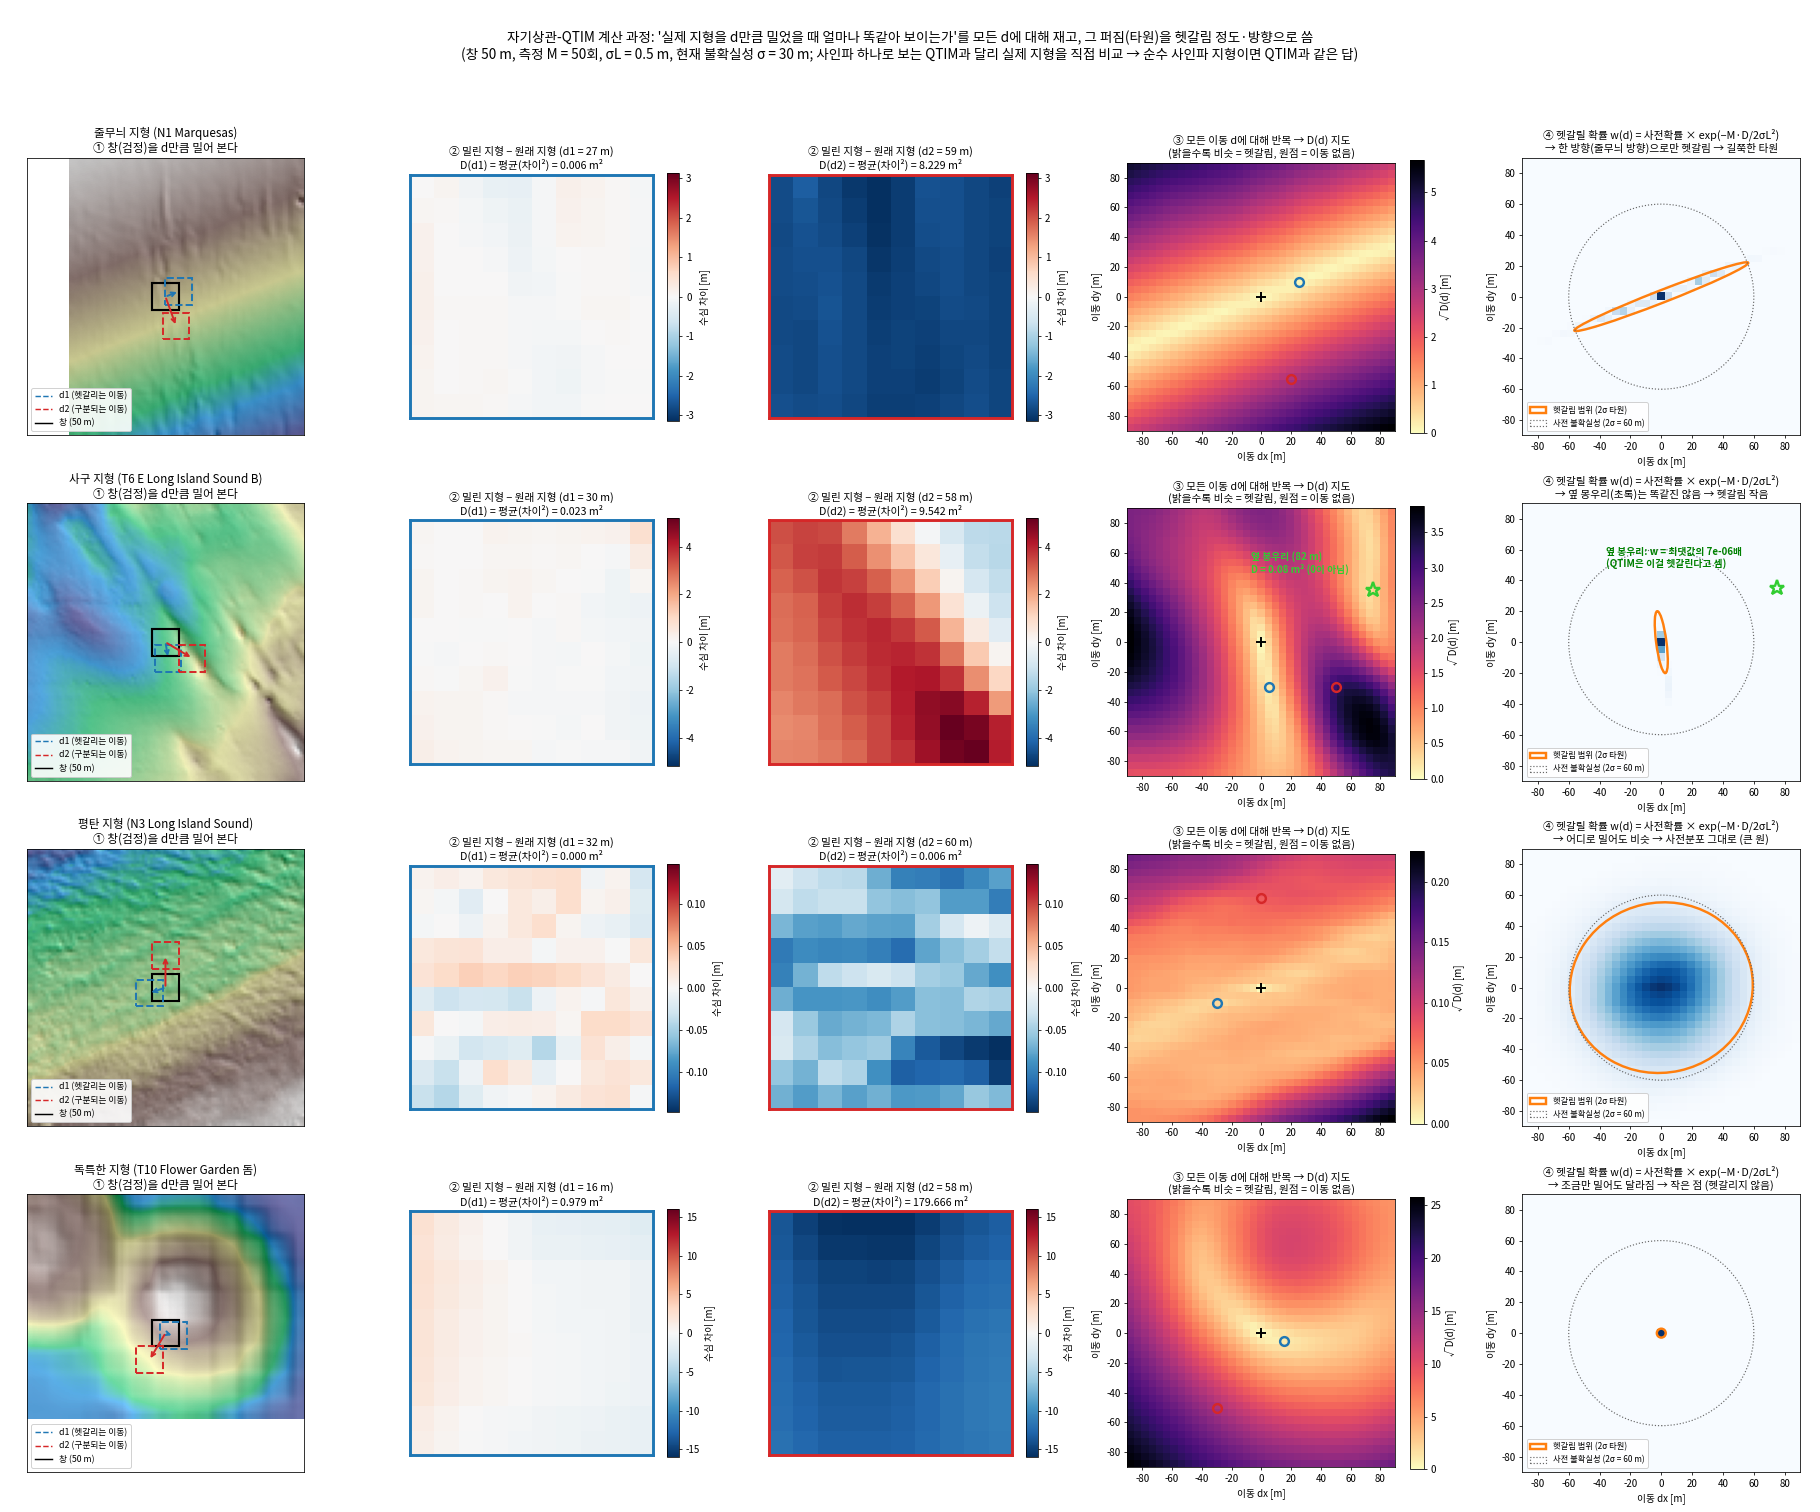
\includegraphics[width=0.92\linewidth]{figs/fig2_ambiguity_placeholder.png}
  \vspace{-5pt}
  \caption{Autocorrelation-based ambiguity on four terrain types (window $w = 50$~m, $M = 50$, $\sigma_L = 0.5$~m, $\sigma = 30$~m). From left to right: terrain with the analysis window shifted by an indistinguishable offset $\bd_1$ and a distinguishable offset $\bd_2$; the corresponding elevation differences; the map of $\sqrt{D(\bx,\bd)}$ over all offsets; and the offset posterior $\pi_\sigma$ with its $2\sigma$ ellipse. Linear stripes leave the along-stripe offset ambiguous, sand waves create isolated secondary minima at neighboring crests, flat terrain leaves the prior unchanged, and a unique dome collapses the posterior to a point.}
  \label{fig:ambiguity}
  \vspace{-10pt}
\end{figure*}

\subsection{Properties}
The following proposition shows that the proposed information is consistent with the Fisher information when the uncertainty is small.

\begin{proposition}\label{prop:fisher}
Let $h$ be four times continuously differentiable on a neighborhood of $\mathcal{W}(\bx)$, and let $G(\bx) = \frac{1}{|\mathcal{W}|}\int_{\mathcal{W}(\bx)} \nabla h(\bq)\nabla h(\bq)^\top d\bq$. Then, for a fixed $M$,
\begin{equation}
  \JA(\bx;\sigma) = \frac{1}{\sigma_L^2}\,G(\bx) + O(\sigma^2) \quad \text{as } \sigma \to 0,
\end{equation}
i.e., $\JA$ converges to the window-averaged Fisher information $\JFbar(\bx)$.
\end{proposition}

\begin{proof}
By Taylor expansion, $h(\bq+\bd) - h(\bq) = \nabla h(\bq)^\top\bd + \frac{1}{2}\bd^\top\nabla^2 h(\bq)\bd + O(\|\bd\|^3)$, so that $D(\bx,\bd) = \bd^\top G\bd + c_3(\bd) + O(\|\bd\|^4)$, where $c_3$ is a homogeneous cubic form. Without the higher-order terms, \eqref{eq:posterior} is a zero-mean Gaussian with precision $A = \sigma^{-2}I + (M/\sigma_L^2)G$, and \eqref{eq:Jac} gives exactly $G/\sigma_L^2$. Since $\pi_\sigma$ concentrates on $\|\bd\| = O(\sigma)$, the first-order perturbation of the second moment by the odd form $c_3$ vanishes, and the remaining perturbations are $\delta\Sigma = O(M\sigma^6/\sigma_L^2) + O(M^2\sigma^8/\sigma_L^4)$. With $\|A\| = O(\sigma^{-2})$, $\Sigma_\sigma^{-1} = A - A\,\delta\Sigma\,A + \ldots = A + O(M\sigma^2)$. Since $G \succeq 0$, the projection $[\cdot]_+$ in~\eqref{eq:Jac} changes the result by at most the same order, and dividing by $M$ yields the claim.
\end{proof}

\begin{remark}\label{rem:periodic}
For the sand-wave field $h(\bq) = a\cos(2\pi\,\mathbf{n}^\top\bq/\lambda)$ and a window spanning several wavelengths, \eqref{eq:D} becomes $D(\bx,\bd) = a^2\big(1 - \cos(2\pi\,\mathbf{n}^\top\bd/\lambda)\big)$, which vanishes at every $\bd = m\lambda\mathbf{n}$ and is independent of the along-crest component of $\bd$. If $\sigma \gg \lambda$, $\pi_\sigma$ consists of narrow peaks at $m\lambda\mathbf{n}$ weighted by the prior, so that $\Sigma_\sigma \approx \sigma^2 I$ and $\JA \approx 0$, whereas $\JFbar$ is independent of $\sigma$. If $\sigma \ll \lambda$, Proposition~\ref{prop:fisher} gives $\JA \approx \JFbar$. Repetitive terrain is thus treated as uninformative until the belief becomes narrow enough to resolve its period, which is exactly the behavior required for reliable TRN.
\end{remark}

\subsection{Multi-Scale Precomputation}
Because~\eqref{eq:D}--\eqref{eq:Jac} depend only on the map and the belief size, $\JA$ is precomputed offline on a grid of map nodes $\bx$ and a finite set of belief levels $\mathcal{S} = \{\sigma_1 > \cdots > \sigma_L\}$. For each offset $\bd$ on a square grid with spacing $\Delta_d = \max(\Delta_h, \sigma/5)$ within $\|\bd\| \le 3\sigma$, where $\Delta_h$ is the map resolution, the difference map $(h(\cdot + \bd) - h(\cdot))^2$ is box-filtered over the window, which yields $D(\cdot,\bd)$ for all map nodes at once. The moments~\eqref{eq:second_moment} are accumulated over the offsets with a streaming log-sum-exp to avoid underflow, and $\Delta_d^2/12$ is added to the diagonal to account for the offset-grid resolution. The cost is $O(N_d N_h)$ per level for $N_d$ offsets and $N_h$ map cells and is independent of the planner. At run time, $\JA(\bx;\sigma)$ is obtained by a nearest-node lookup and a linear interpolation in $\log\sigma$ between adjacent levels, with $\sigma$ clipped to $[\sigma_L, \sigma_1]$. In this study, $\Delta_h = 5$~m, $w = 50$~m, $M = 33$ (the number of pings over $50$~m at $1.5$~m/s and $1$~Hz), $\sigma_L = 0.5$~m, $\mathcal{S} = \{50, 35, 20, 10, 5\}$~m, and the map nodes are spaced by $20$~m.

%% ---------------------------------------------------------------
%%  SECTION V -- AC-MPPI
%% ---------------------------------------------------------------
\section{Autocorrelation-Informed MPPI}
\label{sec:mppi}
The proposed planner, referred to as the autocorrelation-informed MPPI (AC-MPPI), is shown in Fig.~\ref{fig:architecture}. At every replanning instant, it receives the PF estimate $\hat{\bx}$ and covariance $P$, samples heading-rate sequences, rolls them out with an AUV maneuvering model, predicts the covariance at arrival using $\JA$, and passes the optimized heading-rate command to the heading autopilot of the vehicle.

\begin{figure}
  \centering
  % TODO: block diagram: PF (x_hat, P) -> AC-MPPI [sampling -> REMUS horizontal rollouts -> belief-dependent
  %       covariance prediction with J_AC lookup (offline multi-scale maps) -> cost -> weighted update]
  %       -> (psi_ref, r_ref) -> heading / depth autopilots -> 6-DOF REMUS 100 -> altimeter, DVL -> PF.
  \figbox{Fig.~3 placeholder: overall architecture of the proposed framework.}{3.6cm}
  \caption{Overall architecture of the proposed framework. The autocorrelation information maps are precomputed offline at multiple belief levels. At each replanning instant, AC-MPPI evaluates sampled heading-rate sequences by rolling out the AUV maneuvering model and predicting the covariance at arrival with the belief-dependent information, and the resulting heading command is tracked by the autopilot of the vehicle.}
  \label{fig:architecture}
  \vspace{-10pt}
\end{figure}

\subsection{Rollout Model}
For the rollouts, \eqref{eq:kinetics} is reduced to the horizontal plane by setting $w = p = q = 0$ and $\phi = \theta = 0$ and fixing the propeller speed, which yields the surge--sway--yaw model
\begin{equation}
  M_h\dot{\nu}_h + C_h(\nu_h)\nu_h + D_h(\nu_h)\nu_h = \tau_h(\delta_r),
  \label{eq:horizontal}
\end{equation}
where $\nu_h = [u, v, r]^\top$ and the matrices are the corresponding rows and columns of~\eqref{eq:kinetics}. The decision variable is a heading-rate sequence $U = (u_0, \ldots, u_{N-1})$, $|u_n| \le r_{\max}$, each held for $\Delta t$. Within a rollout, the heading autopilot of the vehicle tracks $\psi_{\mathrm{ref}}(t) = \psi_0 + \int_0^t u\,dt'$ with $r_{\mathrm{ref}} = u$, so that the rollout reproduces the closed-loop response of the vehicle to the command. Each rollout is integrated with a step of $0.5$~s from the current estimate and velocity and is evaluated at its step points $\bp_1, \ldots, \bp_T$ with durations $\tau_1, \ldots, \tau_T$. A rollout that passes within $r_a$ of the goal is terminated there, and otherwise the path is completed by a straight segment to the goal sampled every $25$~m, so that every candidate is evaluated up to arrival.

\subsection{Belief-Dependent Covariance Prediction}
Along each rollout, the covariance is predicted from $P_0 = P$ with the number of pings $n_t = \tau_t / T_p$ in each segment as
\begin{subequations}\label{eq:prediction}
\begin{align}
  P_{t|t-1} &= P_{t-1} + n_t\,\sigma_q^2 I, \label{eq:pred_a} \\
  \sigma_t &= \sqrt{\tfrac{1}{2}\tr P_{t|t-1}}, \label{eq:pred_b} \\
  \bar{J}_t &= \textstyle\sum_{j=0}^{4} c_j\, \JA(\bp_t + \bs_j;\, \sigma_t), \label{eq:pred_c} \\
  P_t &= \big( P_{t|t-1}^{-1} + n_t\,\bar{J}_t \big)^{-1}, \label{eq:pred_d}
\end{align}
\end{subequations}
where $\bs_0 = \mathbf{0}$ and $\bs_{\pm i} = \pm\sqrt{3\mu_i}\,\mathbf{e}_i$ are the sigma points of $P_0$ with eigenpairs $(\mu_i, \mathbf{e}_i)$, $c_0 = 1/3$, and $c_{\pm i} = 1/6$. The sigma points average the information over the region where the vehicle may actually be, so that a narrow informative feature that an offset vehicle would miss does not attract the planner. The belief level~\eqref{eq:pred_b} is taken from the predicted covariance itself, which makes the information depend on the path history: repetitive terrain contributes to~\eqref{eq:pred_d} only after the predicted belief has been narrowed by unambiguous terrain earlier along the same rollout. The cost of a sequence $U$ is
\begin{equation}
  S(U) = \tr P_T + \alpha\, T(U) + c_{\mathrm{out}}\,\mathbb{1}_{\mathrm{out}}(U),
  \label{eq:cost}
\end{equation}
where $T(U) = \sum_t \tau_t$ is the time to arrival and $\mathbb{1}_{\mathrm{out}}$ penalizes rollouts that leave the map. Replacing $\JA$ in~\eqref{eq:pred_c} by the point Fisher information~\eqref{eq:fisher} at the beam footprint yields the Fisher-based counterpart used as a baseline in Section~\ref{sec:results}.

\subsection{MPPI Update}
At each replanning instant, $K$ sequences $U^k = \mathrm{clip}(\bar{U} + \boldsymbol{\epsilon}^k)$ with $\boldsymbol{\epsilon}^k \sim \mathcal{N}(\mathbf{0}, \sigma_u^2 I)$ are sampled around the nominal sequence $\bar{U}$, which is included unperturbed together with the direct-to-goal sequence $U_{\mathrm{dir}}$. The sequences are weighted by
\begin{equation}
  \rho^k = \frac{\exp\!\big(-(S(U^k) - S_{\min})/\gamma\big)}{\sum_{l=1}^{K}\exp\!\big(-(S(U^l) - S_{\min})/\gamma\big)},
  \label{eq:weights}
\end{equation}
where the temperature $\gamma$ is determined by bisection so that the ESS $(\sum_k (\rho^k)^2)^{-1}$ equals $0.1K$, which keeps the update insensitive to the scale of the cost. The nominal sequence is updated as
\begin{equation}
  \bar{U} \leftarrow \mathrm{clip}\Big(\bar{U} + \textstyle\sum_{k=1}^{K}\rho^k\,\boldsymbol{\epsilon}^k\Big),
  \label{eq:update}
\end{equation}
and the cheaper of $\bar{U}$ and $U_{\mathrm{dir}}$ is executed. The first command is applied as $r_{\mathrm{ref}} = u_0$ and $\psi_{\mathrm{ref}}(t) = \psi(t_r) + u_0(t - t_r)$ to the heading autopilot of the 6-DOF vehicle until the next replanning at $t_r + T_r$, and $\bar{U}$ is shifted by one step as a warm start. The complete procedure is summarized in Algorithm~\ref{alg:acmppi}.

\begin{algorithm}[t]
\caption{AC-MPPI at a replanning instant}
\label{alg:acmppi}
\begin{algorithmic}[1]
\REQUIRE PF estimate $\hat{\bx}$ and covariance $P$, heading $\psi$, velocity $\nu_h$, goal $\bg$, nominal sequence $\bar{U}$, precomputed $\JA(\cdot;\sigma)$ for $\sigma \in \mathcal{S}$
\STATE Sample $\boldsymbol{\epsilon}^k$ and form $U^k$, $k = 1,\ldots,K$; include $\bar{U}$ and $U_{\mathrm{dir}}$
\FOR{$k = 1$ \TO $K$ \textbf{in parallel}}
  \STATE Roll out~\eqref{eq:horizontal} under $U^k$ from $(\hat{\bx}, \psi, \nu_h)$; append the straight segment to $\bg$
  \STATE $P_0 \leftarrow P$; \textbf{for} $t = 1,\ldots,T$: predict $P_t$ by~\eqref{eq:prediction}
  \STATE Evaluate $S(U^k)$ by~\eqref{eq:cost}
\ENDFOR
\STATE Find $\gamma$ such that the ESS of~\eqref{eq:weights} equals $0.1K$
\STATE Update $\bar{U}$ by~\eqref{eq:update}; \textbf{if} $S(U_{\mathrm{dir}}) \le S(\bar{U})$ \textbf{then} $\bar{U} \leftarrow U_{\mathrm{dir}}$
\STATE Apply $u_0$ for $T_r$; shift $\bar{U}$ by one step
\end{algorithmic}
\end{algorithm}

%% ---------------------------------------------------------------
%%  SECTION VI -- SIMULATION RESULTS
%% ---------------------------------------------------------------
\section{Simulation Results}
\label{sec:results}

\subsection{Simulation Setup}
\subsubsection{Vehicle and navigation}
The 6-DOF REMUS~100 model~\eqref{eq:kinematics}--\eqref{eq:kinetics} was simulated at $10$~Hz with a constant propeller speed of $896$~rpm, which yields a cruise speed of $1.5$~m/s. The vehicle followed the seafloor at an altitude of $8$~m, where the depth set-point was given by the altimeter and raised for the shallowest map elevation within $200$~m ahead of and $100$~m around the estimated position. Navigation ran at $1$~Hz with known heading and without currents. The simulation parameters are summarized in Table~\ref{tab:params}.

\begin{table}
\caption{Simulation and planner parameters.}
\centering
\footnotesize
\begin{tabular}{l l}
\hline
\textbf{Parameter} & \textbf{Value} \\ \hline
Vehicle speed / altitude & $1.5$~m/s / $8$~m \\
Altimeter rate / noise $\sigma_z$ & $1$~Hz / $0.3$~m \\
DR noise $\sigma_w$ & $0.2$~m per ping and axis \\
Initial uncertainty $\sigma_0$ & $50$~m \\
PF particles / $\sigma_L$ / $\sigma_q$ & $5000$ / $0.5$~m / $0.3$~m \\
Route length / arrival radius $r_a$ / $T_{\max}$ & $1.4$~km / $10$~m / $2350$~s \\
MPPI samples $K$ / step $\Delta t$ / horizon $N$ & $512$ / $10$~s / $40$ ($400$~s) \\
$\sigma_u$ / $r_{\max}$ / replanning $T_r$ & $2^\circ$/s / $5^\circ$/s / $10$~s \\
Time weight $\alpha$ & $0.03$ \\
A* grid / information weight $\lambda$ & $20$~m / $8$ \\
\hline
\end{tabular}
\label{tab:params}
\vspace{-15pt}
\end{table}

\subsubsection{Terrains and routes}
Eight $2$~km~$\times$~$2$~km crops of the NOAA BlueTopo bathymetry compilation\footnote{\url{https://nauticalcharts.noaa.gov/data/bluetopo.html}} with source resolutions of $4$--$16$~m were resampled to $5$~m resolution, using only crops covered by a single survey to avoid interpolation artifacts. As listed in Table~\ref{tab:terrain}, they include linear stripes (S1), a slope band (S2), domes with an escarpment (S3), sand-wave fields (S4--S6 and S8), and patchy hard-bottom texture (S7). One test route per terrain was defined by a fixed rule (Fig.~\ref{fig:terrains}): a length of $1.4$~km ($28\sigma_0$), a heading within $\pm 10^\circ$ of the dominant feature direction obtained from the terrain structure tensor, and, among such routes, the straight corridor with the largest mean expected error after one pass, subject to an informative area within $300$~m of the route. The goal lies in an informative area on five terrains and in an ambiguous area on three. The routes thus represent missions in which the direct path runs along ambiguous structure while unambiguous terrain is reachable, which is the setting targeted by active localization; this selection favors information-aware methods over straight-line guidance by design. For each terrain, $30$ initial offsets $\mathbf{e}_0 \sim \mathcal{N}(\mathbf{0}, 50^2 I)$ were drawn and shared by all methods together with the sensor-noise and PF random streams, so that every comparison is paired.

\begin{figure*}
  \centering
  % TODO: single English figure with the eight test terrains (S1-S8): bathymetry + route (top), E_AC map at sigma0 (bottom).
  %       NOTE: the left placeholder (p49) still contains the Hudson shelf-valley terrain, which is not part of this study.
  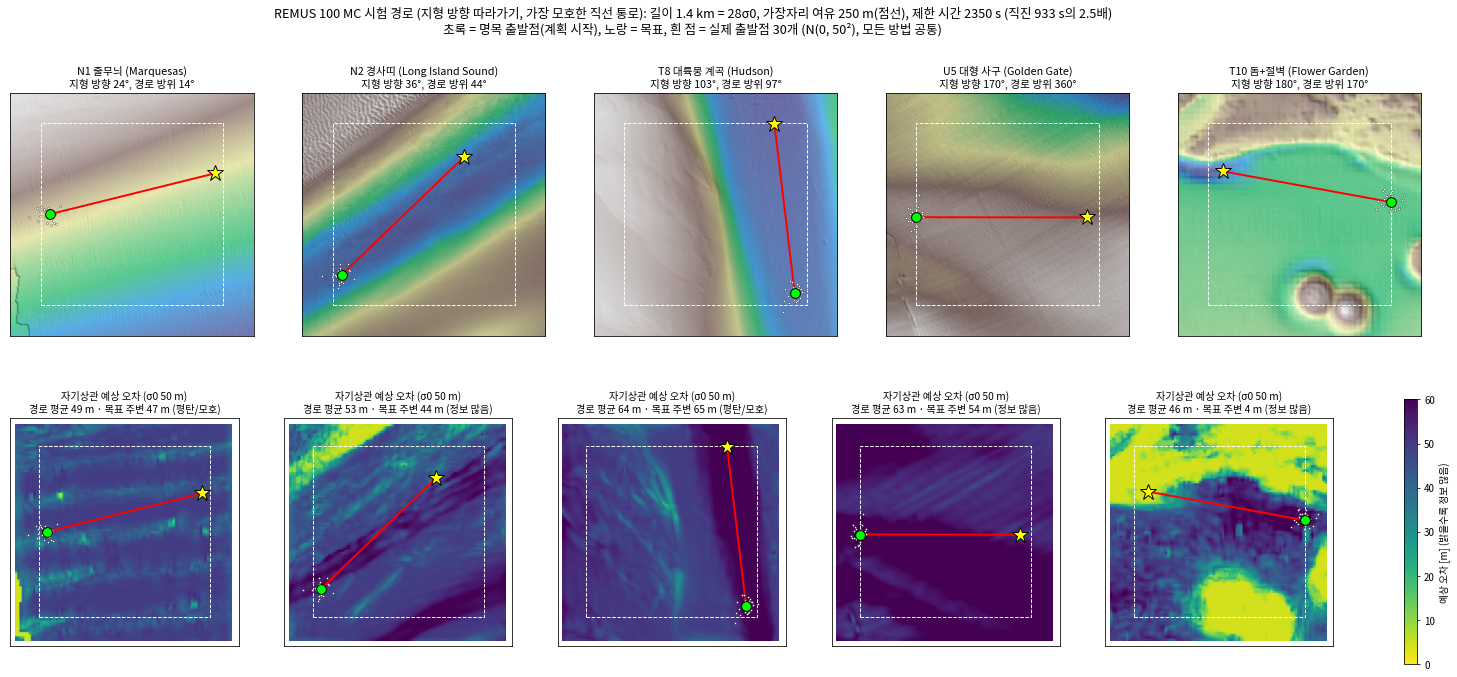
\includegraphics[width=0.49\linewidth]{figs/fig4a_routes_placeholder.png}\hfill
  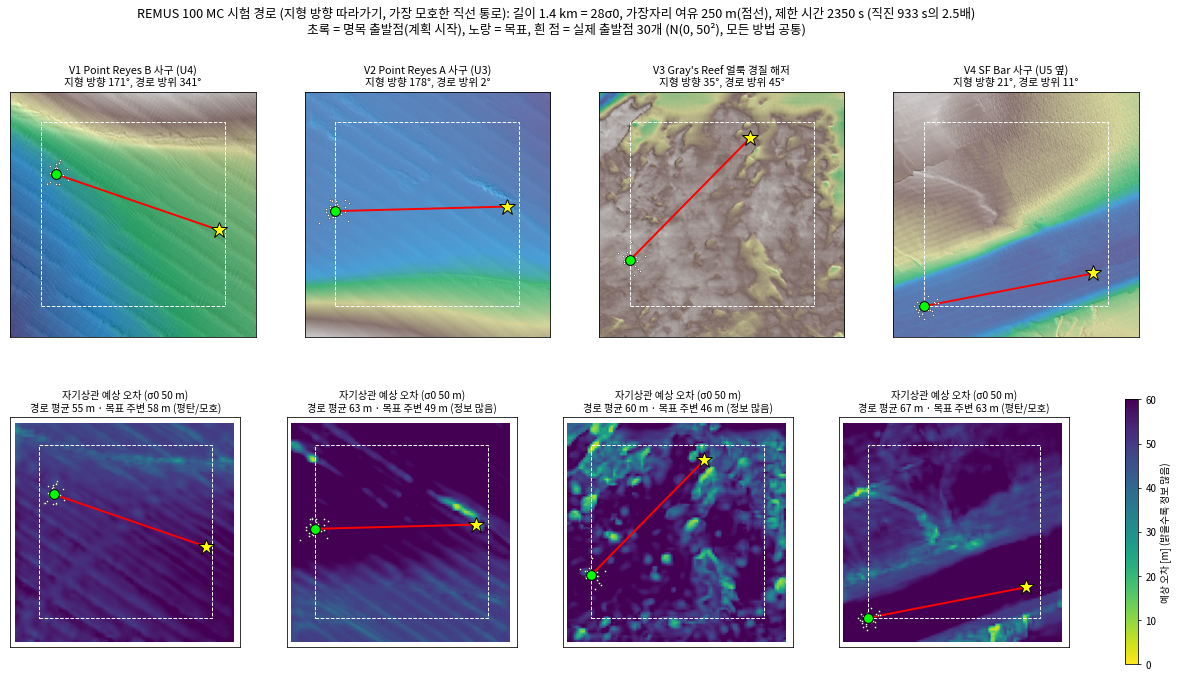
\includegraphics[width=0.49\linewidth]{figs/fig4b_routes_placeholder.png}
  \vspace{-5pt}
  \caption{Eight test terrains with their routes. Top: bathymetry with the nominal start (green), goal (yellow), and the $30$ true start positions (white). Bottom: expected error after one pass at $\sigma_0 = 50$~m computed from the autocorrelation information (brighter is more informative). The routes follow the dominant feature direction along the most ambiguous straight corridor.}
  \label{fig:terrains}
  \vspace{-10pt}
\end{figure*}

\subsubsection{Compared methods}
Six methods were compared under identical vehicle, navigation, and arrival settings. 1) \emph{Straight-LOS}: line-of-sight (LOS) guidance along the straight line to the goal with an $80$~m lookahead, a straight final approach within $150$~m, and a go-around after a missed arrival. 2) \emph{Fisher-A*}: an information-weighted A* path planned once from the initial estimate on an $8$-connected $20$~m grid with the edge cost (length)$\times(1 + \lambda u)$, where $u \in [0,1]$ is the normalized expected error after one pass, $E_{\mathrm{F}}(\bx) = \sqrt{\tr((\sigma_0^{-2}I + M\JFbar(\bx))^{-1})}$; the path is simplified into waypoints and followed by the same LOS guidance. 3) \emph{AC-A*}: the same planner with $E_{\mathrm{AC}}(\bx) = \sqrt{\tr\Sigma_{\sigma_0}(\bx)}$. 4) \emph{Fisher-MPPI}: AC-MPPI with $\JA$ in~\eqref{eq:pred_c} replaced by the point Fisher information~\eqref{eq:fisher}. 5) \emph{Entropy-MPPI}: the same MPPI with the covariance term in~\eqref{eq:cost} replaced by the expected entropy of the particle belief at arrival, estimated from \tbd{$N_e$} particles subsampled from the PF and \tbd{$N_z$} simulated measurement sequences per rollout~\cite{hoffmann2010mobile, ryan2010particle}. % TODO: make this description match the implemented baseline.
6) \emph{AC-MPPI} (proposed). Methods 2)--4) and 6) form a factorial design that combines two information models with two planners, which separates the contribution of each component. All MPPI variants share $K$, $\Delta t$, $N$, $\sigma_u$, and $\alpha$, which were fixed a priori; their sensitivity is examined in Section~\ref{sec:sensitivity}. The A* planners used $\lambda = 8$; with $\lambda = 2$, their pooled success rates were $90.0\%$ (Fisher-A*) and $90.8\%$ (AC-A*), so the conclusions below do not depend on this choice.

\subsubsection{Metrics}
The success rate, false arrivals, and timeouts were counted as defined in Section~\ref{sec:problem}. The mean arrival time over successful runs, the mean path length, and the root mean square error (RMSE) between the estimated and true trajectories were also reported. Paired differences in success were tested with the exact McNemar test on the discordant pairs, and $95\%$ Wilson confidence intervals (CIs) are given for the pooled success rates. All simulations were executed on \tbd{[CPU model, clock, RAM]}.

\subsection{Overall Performance}
The pooled results over the eight terrains are summarized in Table~\ref{tab:overall}. AC-MPPI succeeded in $234$ of $240$ runs ($97.5\%$), the highest success rate among all methods, and the paired McNemar tests confirmed that its advantage over every baseline is significant. The failures of the baselines differ in kind. Straight-LOS and the two one-shot A* planners failed almost exclusively by false arrival, in $75$, $28$, and $19$ runs, respectively: the PF converged to a wrong hypothesis while reporting a small covariance, and the vehicle stopped at a wrong location without detecting the error. Fisher-MPPI rarely arrived falsely, but it timed out in $28$ runs, because it kept steering toward terrain that its gradient-based prediction considered informative while the actual belief failed to contract. AC-MPPI reduced both failure types simultaneously, with $6$ false arrivals and no timeouts, and it also attained the lowest trajectory RMSE of $23.8$~m.

The improvement is obtained at the cost of a longer mission than straight-line guidance: the mean arrival time increased from $946$~s to $1204$~s and the mean path length from $1414$~m to $1810$~m. Compared with Fisher-MPPI, however, AC-MPPI traveled a shorter mean path ($1810$~m versus $1955$~m) and arrived in a similar time, because the ambiguity-aware prediction does not reward loitering over repetitive terrain.

\begin{table*}
  \centering
  \caption{Pooled Monte Carlo results over eight terrains ($30$ paired runs per terrain, $240$ per method). McNemar: runs in which only AC-MPPI succeeded / only the baseline succeeded, with the exact $p$-value. Planning time: per replanning for MPPI and per plan for A*.}
  \footnotesize
  \setlength{\tabcolsep}{4.5pt}
  \begin{tabular}{l c c c c c c c c}
    \hline
    \textbf{Method} & \textbf{Success [\%] (95\% CI)} & \textbf{False arr.} & \textbf{Timeout} & \textbf{Time [s]} & \textbf{Path [m]} & \textbf{RMSE [m]} & \textbf{Plan. time [ms]} & \textbf{McNemar} \\
    \hline
    Straight-LOS   & $68.8$ ($62.6$--$74.3$) & $75$ & $0$  & $946$  & $1414$ & $32.1$ & -- & $72/3$, $p < 10^{-4}$ \\
    Fisher-A*      & $88.3$ ($83.7$--$91.8$) & $28$ & $0$  & $1175$ & $1752$ & $24.2$ & \tbd{XX} & $27/5$, $p = 1.1\times10^{-4}$ \\
    AC-A*          & $92.1$ ($88.0$--$94.9$) & $19$ & $0$  & $1113$ & $1657$ & $24.0$ & \tbd{XX} & $17/4$, $p = 7.2\times10^{-3}$ \\
    Fisher-MPPI    & $87.1$ ($82.2$--$90.7$) & $3$  & $28$ & $1169$ & $1955$ & $25.8$ & \tbd{XX} & $30/5$, $p = 2.2\times10^{-5}$ \\
    Entropy-MPPI   & \tbd{XX} (\tbd{XX}--\tbd{XX}) & \tbd{XX} & \tbd{XX} & \tbd{XX} & \tbd{XX} & \tbd{XX} & \tbd{XX} & \tbd{XX/XX}, \tbd{$p = $ XX} \\
    \textbf{AC-MPPI (proposed)} & $\mathbf{97.5}$ ($94.7$--$98.8$) & $6$ & $\mathbf{0}$ & $1204$ & $1810$ & $\mathbf{23.8}$ & \tbd{XX} & -- \\
    \hline
  \end{tabular}
  \label{tab:overall}
  \vspace{-10pt}
\end{table*}

\subsection{Per-Terrain Analysis}
The per-terrain results in Table~\ref{tab:terrain} show where the improvement originates. On S3, S6, and S7, where unambiguous terrain lies near the route or around the goal, the four A*- and MPPI-based planners succeeded in every run. On S1 and S2, whose elongated features leave only the along-feature offset ambiguous, any path that crosses the stripes or the band resolves the ambiguity, and these planners succeeded in at least $29$ of $30$ runs, whereas Straight-LOS, traveling along the features, arrived falsely in $17$ and $5$ runs. The differences among the information-aware planners concentrate on the sand-wave fields S4, S5, and S8, where the terrain gradient is large but periodic. There, Fisher-MPPI succeeded in $20$, $12$, and $27$ runs with $28$ timeouts in total, the one-shot A* planners in $17$--$29$ runs with $47$ false arrivals in total, and AC-MPPI in $28$, $28$, and $29$ runs.

The factorial design separates the two components. Replacing the Fisher information by the proposed information raised the success rate from $88.3\%$ to $92.1\%$ with the one-shot A* planner and from $87.1\%$ to $97.5\%$ with MPPI, whereas replacing the A* planner by MPPI changed the success rate from $88.3\%$ to $87.1\%$ with the Fisher information but from $92.1\%$ to $97.5\%$ with the proposed information. The closed-loop planner therefore pays off only in combination with the ambiguity-aware information model. With the Fisher information, replanning from the current belief repeatedly predicts that crossing the sand waves will shrink the covariance, so the vehicle keeps returning to the sand-wave field while the actual belief remains multimodal. With the proposed information, the same field is predicted to be uninformative at a large belief size, so the planner first seeks unambiguous terrain and exploits the sand waves only after the belief has contracted. The one-shot A* planners cannot react to the realized belief: when the true start offset makes the vehicle miss the planned informative area, it continues along the plan and arrives falsely, regardless of the information map used for planning.

\begin{table}
  \centering
  \caption{Successful runs out of $30$ per terrain. Parentheses: false arrivals / timeouts (omitted when zero).}
  \footnotesize
  \setlength{\tabcolsep}{2.2pt}
  \resizebox{\linewidth}{!}{%
  \begin{tabular}{l c c c c c c}
    \hline
    \textbf{Terrain} & \textbf{\makecell{Straight\\-LOS}} & \textbf{\makecell{Fisher\\-A*}} & \textbf{\makecell{AC\\-A*}} & \textbf{\makecell{Fisher\\-MPPI}} & \textbf{\makecell{Entropy\\-MPPI}} & \textbf{\makecell{AC-MPPI\\(prop.)}} \\
    \hline
    S1 Marquesas, FL (stripes)   & $13$ ($17/0$) & $30$ & $30$ & $30$ & \tbd{XX} & $29$ ($1/0$) \\
    S2 Long Isl.\ Sd., NY (slope band) & $25$ ($5/0$) & $30$ & $30$ & $30$ & \tbd{XX} & $30$ \\
    S3 Flower Garden, GoM (domes) & $30$ & $30$ & $30$ & $30$ & \tbd{XX} & $30$ \\
    S4 Golden Gate, CA (sand waves) & $20$ ($10/0$) & $17$ ($13/0$) & $25$ ($5/0$) & $20$ ($0/10$) & \tbd{XX} & $\mathbf{28}$ ($2/0$) \\
    S5 Point Reyes B, CA (sand waves) & $17$ ($13/0$) & $20$ ($10/0$) & $17$ ($13/0$) & $12$ ($0/18$) & \tbd{XX} & $\mathbf{28}$ ($2/0$) \\
    S6 Point Reyes A, CA (sand waves) & $20$ ($10/0$) & $30$ & $30$ & $30$ & \tbd{XX} & $30$ \\
    S7 Gray's Reef, GA (hard bottom) & $29$ ($1/0$) & $30$ & $30$ & $30$ & \tbd{XX} & $30$ \\
    S8 SF Bar, CA (sand waves) & $11$ ($19/0$) & $25$ ($5/0$) & $29$ ($1/0$) & $27$ ($3/0$) & \tbd{XX} & $29$ ($1/0$) \\
    \hline
    Total ($240$) & $165$ & $212$ & $221$ & $209$ & \tbd{XX} & $\mathbf{234}$ \\
    \hline
  \end{tabular}}
  \label{tab:terrain}
  \vspace{-15pt}
\end{table}

\subsection{Illustrative Run}
Fig.~\ref{fig:run} contrasts the failure modes on S5 for one initial offset that was shared by all methods. Straight-LOS and AC-A* traveled along the sand waves and arrived falsely with final errors of $52$~m and $28$~m, respectively. Fisher-A* reached the goal after a $2192$~m detour in $1464$~s. Fisher-MPPI loitered over the sand-wave field around the goal, where its prediction kept promising a covariance reduction, and timed out at $2350$~s after traveling $3511$~m while its filter uncertainty $\sqrt{\tr P}$ remained above $10$~m. AC-MPPI deviated from the direct route early in the mission, its filter uncertainty fell below $10$~m at $588$~s, and it arrived in $1129$~s with an error of $5$~m over a path of $1690$~m.

\begin{figure}
  \centering
  % TODO: English version of results/p54/run_V1.png (true tracks | estimation error | sqrt(tr P) | distance to goal).
  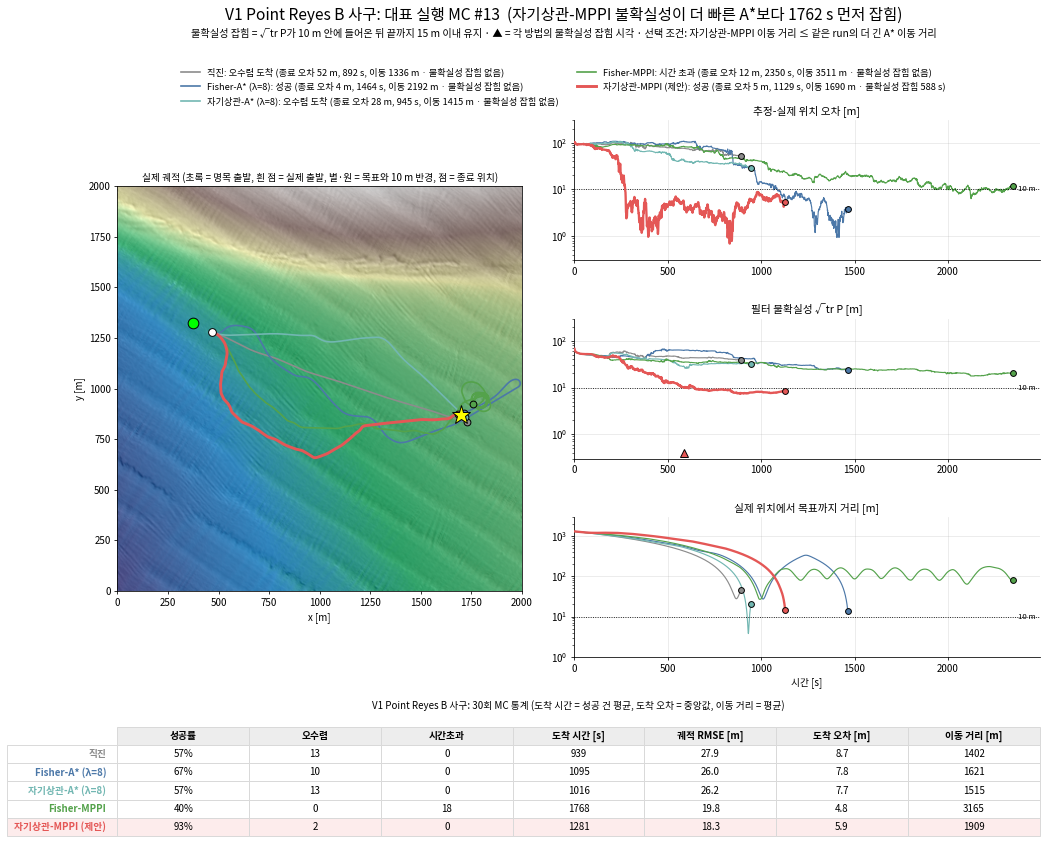
\includegraphics[width=\linewidth]{figs/fig5_run_placeholder.png}
  \vspace{-15pt}
  \caption{Illustrative run on S5 (Point Reyes B), selected to contrast the failure modes of the baselines. Left: true tracks on the bathymetry. Right: estimation error, filter uncertainty $\sqrt{\tr P}$, and true distance to the goal over time.}
  \label{fig:run}
  \vspace{-10pt}
\end{figure}

\subsection{Comparison with Particle-Entropy Planning}
% TODO: rewrite this subsection according to the actual Entropy-MPPI results (success, failure types, planning time).
Entropy-MPPI evaluates the multimodal particle belief directly and therefore does not rely on the Gaussian approximation in~\eqref{eq:prediction}. It achieved a success rate of \tbd{XX}\% with \tbd{XX} false arrivals and \tbd{XX} timeouts (Table~\ref{tab:overall}), while requiring \tbd{XX}~ms per replanning, \tbd{XX} times that of AC-MPPI. \tbd{[Interpret: e.g., whether the subsampled particle set and the limited number of simulated measurement sequences were sufficient to represent the ambiguity on S4, S5, and S8 within the real-time budget.]} In contrast, AC-MPPI moves the evaluation of the ambiguity offline into the multi-scale maps, so that its online cost per rollout remains that of a covariance recursion with table lookups.

\subsection{Parameter Sensitivity}
\label{sec:sensitivity}
The sensitivity of the MPPI planners to the time weight $\alpha$ and the horizon $N\Delta t$ was evaluated on S1--S4 with $20$ additional initial offsets per terrain that were disjoint from the test offsets ($80$ runs per setting), as summarized in Table~\ref{tab:sensitivity}. AC-MPPI attained success rates of $95.0$--$100\%$ over the entire grid. Fisher-MPPI ranged from $83.8\%$ to $98.8\%$ and approached the proposed method only with the largest time weight $\alpha = 0.05$ and the shorter horizon. A larger $\alpha$ suppresses the detours that the overconfident Fisher prediction otherwise sustains, which is consistent with the timeout failures observed above. The proposed information model thus removes the need to tune the time weight against the terrain ambiguity.
% TODO (before submission): run Fisher-MPPI with alpha = 0.05 / horizon 400 s on all eight terrains with the test offsets
%       and report it, since a reviewer will ask whether a tuned Fisher-MPPI closes the gap on S5 and S8.

\begin{table}
  \centering
  \caption{Success rate [\%] of the MPPI planners on S1--S4 for different time weights $\alpha$ and horizons ($80$ runs per setting, offsets disjoint from the test set).}
  \footnotesize
  \setlength{\tabcolsep}{5pt}
  \begin{tabular}{c c c c c}
    \hline
    & \multicolumn{2}{c}{\textbf{Fisher-MPPI}} & \multicolumn{2}{c}{\textbf{AC-MPPI}} \\
    $\alpha$ & $400$~s & $600$~s & $400$~s & $600$~s \\
    \hline
    $0.01$ & $85.0$ & $83.8$ & $98.8$ & $95.0$ \\
    $0.02$ & $85.0$ & $88.8$ & $100.0$ & $97.5$ \\
    $0.03$ & $86.2$ & $90.0$ & $98.8$ & $100.0$ \\
    $0.05$ & $98.8$ & $91.2$ & $100.0$ & $97.5$ \\
    \hline
  \end{tabular}
  \label{tab:sensitivity}
  \vspace{-15pt}
\end{table}

\subsection{Computation Time}
% TODO: fill in after the timing runs.
Precomputing $\JA$ at the five belief levels took \tbd{XX}~s per $2$~km~$\times$~$2$~km map, which is performed once before the mission. The online planning times are listed in Table~\ref{tab:overall}. AC-MPPI required \tbd{XX}~ms per replanning on average (\tbd{XX}~ms at most), comparable to the \tbd{XX}~ms of Fisher-MPPI because both evaluate a covariance recursion along each rollout and differ only in the information lookup, and well within the replanning period of $T_r = 10$~s. Entropy-MPPI required \tbd{XX}~ms.

%% ---------------------------------------------------------------
%%  SECTION VII -- CONCLUSION
%% ---------------------------------------------------------------
\section{Conclusion}
\label{sec:conclusion}
This paper presented an ambiguity-aware active localization framework for terrain-referenced navigation of AUVs that integrates an autocorrelation-based terrain information model into MPPI control. The information model evaluates the local terrain autocorrelation under the current belief size, retains only the information that remains unambiguous, and reduces to the Fisher information when the uncertainty is small. Precomputed at multiple belief scales, it enables a belief-dependent covariance prediction along rollouts of an AUV maneuvering model at the cost of a Fisher information map. Monte Carlo simulations with a 6-DOF REMUS~100 model on eight real bathymetric maps showed that the proposed AC-MPPI achieved a $97.5\%$ success rate, reducing both the false arrivals of straight-line and one-shot A* guidance and the timeouts of Fisher-based MPPI, and that, unlike the Fisher-based planner, its performance was insensitive to the time weight and the horizon on the terrains examined. The factorial comparison further showed that the benefit of closed-loop planning materializes only when it is combined with the ambiguity-aware information. The present study assumed a known heading, no ocean currents, and an error-free prior map, approximated the belief by an isotropic size in the information lookup, and was conducted in simulation. Future work will extend the information model to anisotropic beliefs and map uncertainty and validate the framework in field experiments.

\balance
\bibliographystyle{IEEEtran}
\bibliography{ref}

\end{document}
